\documentclass[11pt]{article}

\usepackage[T1]{fontenc}
\usepackage[utf8]{inputenc}
\usepackage{graphicx}
\usepackage{amsmath}
\usepackage{amssymb}
\usepackage{amsfonts}




\begin{document}
\maketitle

\newpage
\part{Wymagania}


\newpage
\part{Opowieść}

\paragraph{}
W początkach roku 1878\cite{a}, kiedy świat polityczny zajmował się pokojem san-stefańskim, 
wyborem nowego papieża albo szansami europejskiej wojny, warszawscy kupcy tudzież inteligencja pewnej 
okolicy Krakowskiego Przedmieścia niemniej gorąco interesowała się przyszłością galanteryjnego sklepu pod firmą J. Mincel i S. Wokulski.
W renomowanej jadłodajni, gdzie na wieczorną przekąskę zbierali się właściciele składów bielizny i składów win, 
fabrykanci powozów i kapeluszy, poważni ojcowie rodzin utrzymujący się z własnych funduszów i posiadacze kamienic bez zajęcia, 
równie dużo mówiono o uzbrojeniach Anglii(równanie(\ref{jeden})), jak o firmie J. Mincel i S. Wokulski. Zatopieni w kłębach dymu cygar i pochyleni nad butelkami 
z ciemnego szkła, obywatele tej dzielnicy jedni zakładali się o wygranę lub przegranę Anglii(równanie(\ref{dwa})), drudzy o bankructwo Wokulskiego; 
jedni nazywali geniuszem Bismarcka, drudzy - awanturnikiem Wokulskiego; jedni krytykowali postępowanie prezydenta MacMahona, 
inni twierdzili, że Wokulski jest zdecydowanym wariatem, jeżeli nie czymś gorszym...
Pan Deklewski, fabrykant powozów, który majątek(rys(\ref{rysunekjeden})) i stanowisko zawdzięczał wytrwałej pracy w jednym fachu, 
tudzież radca Węgrowicz, który od dwudziestu lat był członkiem - opiekunem jednego i tego samego Towarzystwa Dobroczynności, 
znali S. Wokulskiego\cite{b} najdawniej i najgłośniej przepowiadali mu ruinę(rys(\ref{rysunekdwa})).\\
- Na ruinie bowiem i niewypłacalności - mówił pan Deklewski - musi skończyć człowiek, który nie pilnuje się jednego fachu i nie umie uszanować darów łaskawej fortuny.\\
Zaś radca Węgrowicz po każdej również głębokiej sentencji swego przyjaciela dodawał:\\
- Wariat! wariat!... Awanturnik!... Józiu, przynieś no jeszcze piwa. A która to butelka?\\
- Szósta, panie radco. Służę piorunem!... - odpowiadał Józio.\\
- Już szósta?... Jak ten czas leci!... Wariat! Wariat! - mruczał radca Węgrowicz.\\
Dla osób posilających się w tej co radca jadłodajni, dla jej właściciela, subiektów i chłopców przyczyny klęsk mających paść na S. Wokulskiego
i jego sklep galanteryjny były tak jasne jak gazowe płomyki oświetlające zakład. 
Przyczyny te tkwiły w niespokojnym charakterze, w awanturniczym życiu, zresztą w najświeższym postępku człowieka, 
który mając w ręku pewny kawałek chleba i możność uczęszczania do tej oto tak przyzwoitej restauracji, dobrowolnie wyrzekł się restauracji, 
sklep zostawił na Opatrzności boskiej, a sam z całą gotówką odziedziczoną po żonie pojechał na turecką wojnę robić majątek.
\newpage
\part{Równania}




\newline
\begin{equation}
\label{jeden}
f(x) = ax^2 + bx + c,
\end{equation}

\newline
\begin{eqnarray}
\label{dwa}
a^ 2
x^ {ab}
\end{eqnarray}

\newline
\begin{equation}
f(x) = \left\lbrace
\begin{array}{rcl}
-x^2 & \text{dla} & x < 0,\nonumber\\
\sqrt{x} + \sin x & \text{dla} & x > 0. \nonumber
\end{array}
\right. \nonumber
\end{equation}

\newpage
\part{Obrazki}
\\
\begin{figure}[h]
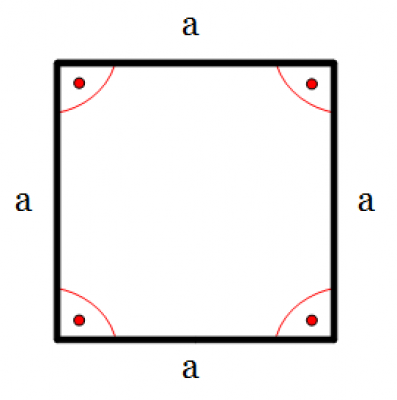
\includegraphics
[width=7cm]{kwadrat}
\caption{Rys(1): Rysunek kwadratu}
\label{rysunekjeden}
\end{figure}

\begin{figure}[h]
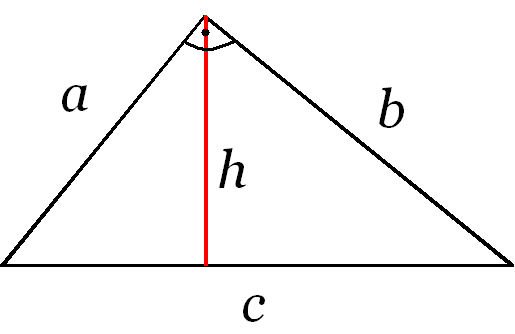
\includegraphics
[width=7cm]{trojkat}
\caption{Rys(2):Rysunek trójkąta}
\label{rysunekdwa}
\end{figure}

\newpage
\part{Tabela}

\\
x=\left[ \begin{array}{cccc}
1 & 2  & 3 \\
4} & 5  & 6 \\
\vdots  & \ddots & \vdots \\
7 & 8  & 9
\end{array} \right]

\newpage
\begin{thebibliography}{9}
\bibitem{a}
Bolesław Prus,
\emph{Lalka}.
1994.
\bibitem{b}
Bolesław Prus,
\emph{Kamizelka}.
1997.
\end{thebibliography}


\end{document}